\documentclass{exam}

\pagenumbering{gobble}
\usepackage{graphicx} %for graphix
\usepackage{titling}
\setlength{\droptitle}{-8ex}
\pretitle{\begin{flushleft}\Large\bfseries}
\posttitle{\par\end{flushleft}}
\preauthor{\begin{flushleft}\Large}
\postauthor{\end{flushleft}}
\predate{\begin{flushleft}}
\postdate{\end{flushleft}}
\usepackage{enumerate} %for alphabetized lists
\usepackage{amsmath}
\usepackage{multicol} %for multiple columns
\usepackage{systeme} %systems of equations
\renewcommand{\questionshook}{\setlength{\itemsep}{15pt}} %controls space betweenites

%fromhttps://texblog.org/2012/06/25/adding--lines--for--taking--handwritten--notes--in--latex/
\usepackage{pgffor, ifthen}
\newcommand{\notes}[3][\empty]{%q
   vspace{10pt}\\
    \foreach \n in {1,...,#2}{%
        \ifthenelse{\equal{#1}{\empty}}
            {\rule{#3}{0.5pt}\\}
            {\rule{#3}{0.5pt}\vspace{#1}\\} 
        }
}

\title{Problem set \#6}

\author{ \textbf{Name: }  \enspace\hrulefill \\ Precalculus \\ Herbert H. Lehman High School } 


\begin{document}
\maketitle
\thispagestyle{empty}

\noindent\textbf{Be sure to...} Do all work in your notebook.  If you don't complete work in class, finish at home. Submit on Google Classroom.
\begin{questions}
\question 
For the matrices below, \textbf{be sure to} (i) find the determinant, showing all work, then (ii) check your answer using the \textbf{determinant calculator} on Google Classroom.  If you got the wrong answer, double check your work and write a sentence explaining what you did wrong:

\begin{parts}
\part
$
A = \begin{bmatrix}
1 & 4 & -2 \\
3 & 2 & 0 \\
-1 & 4 & 3
\end{bmatrix}
$
\vspace{\stretch{1}}
\part

$
B = \begin{bmatrix}
2 & 6 & 5 & 2 \\
2 & 7 & 3 & 6 \\
1 & 5 & 0 &1 \\
3 & 7 & 0 & 7
\end{bmatrix}
$
\vspace{\stretch{1}}

\end{parts}
\question 
%question adapted from: http://linear.ups.edu/fcla/section-WILA.html 
Ashley owns a factory that makes trail mix.  Her factory makes three kinds of trail mix: \textit{bulk}, \textit{standard}, and \textit{fancy.} The trail mix uses three ingredients--raisins, peanuts, and chocolate chips. The table below provides information about how much of each ingredient is used for each variety:

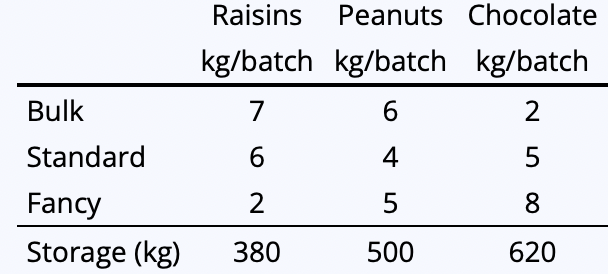
\includegraphics[scale=0.5]{table.png}

As seen in the table, the factor has room to store in the following amounts: 380 kilograms of raisins, 500 kilograms of peanuts and 620 kilograms of chocolate chips.    Ashley asks you  to help determine how much she should make of each mix so that no ingredients are left over at the end of the day.

\textbf{Be sure to...}
\begin{enumerate}[a.]
\item write a system of equations that goes along with this problem
\item Use your linear algebra skills to determine how much of each mix Ashley should make. Feel free to use the  \textbf{determinant and adjugate calculators} on Google Classroom!
\end{enumerate}

\end{questions}

\end{document}